\documentclass[twocolumn]{article}
\usepackage{calc}
\usepackage{ifthen}
\usepackage[margin=0.5in]{geometry}
\usepackage{amsmath,amsthm,amsfonts,amssymb}
\usepackage{amsfonts}
\usepackage{color,overpic}
\usepackage{hyperref}
\usepackage{array} 
\usepackage{amstext}
\usepackage{amsmath}
\usepackage{enumitem}
\usepackage{graphicx}
\usepackage{caption}
\usepackage{natbib}
\usepackage{framed}
\usepackage{float}
%\usepackage[]{algorithm2e}
\usepackage{algpseudocode} 
\usepackage{algorithmicx}
\usepackage{tabto}
\usepackage{amsmath}

\newenvironment{Figure}
  {\par\medskip\noindent\minipage{\linewidth}}
  {\endminipage\par\medskip}
  
\numberwithin{equation}{section}

\NumTabs{10}

% Turn off header and footer
\pagestyle{empty}
\setlist[itemize]{leftmargin=*} % set itemise indentation to leftmargin
\setlist[enumerate]{leftmargin=*}

\setlist[itemize]{itemsep=0mm}
\setlist[enumerate]{itemsep=0mm}

\title{Inverse Problem}
\date{\vspace{-6ex}}

\newcommand*\conj[1]{\overline{#1}}
\newcommand*\mean[1]{\overline{#1}}

% -----------------------------------------------------------------------

\begin{document}
\maketitle





\section{Inverse Problem Formulation}
\begin{framed}
An inverse problem is the process of calculating from a set of observations $d$ the causal factors $m$ that produced them.
$$ \mathbf{d} = G(\mathbf{m}) \mapsto \mathbf{m}=G^{-1}(\mathbf{d})$$
Where $G$ is known as the forward model.
\end{framed}



	\subsection{Classification}
\begin{itemize}
	\item \textbf{Linear vs Non-linear}: if the forward model is linear ($\ \mathbf{d} = \mathbf{G}\mathbf{m}$) or not.
	\item \textbf{Well-posed}: a problem is well posed when a solution (1) exist, (2) is unique and (3) change continuously with initial condition.
	\item \textbf{Well-conditioned}: When a small error in the initial data does not result in much larger errors in the answers, the problem is said to be well-conditioned.  Even if a problem is well-posed, it may still be ill-conditioned. This is evaluated using the condition number (subsection~\ref{subsec:Condition_number})
	\item \textbf{Under vs. Overdetermined}: When more equations than unknowns, the system is overdetermined (more than one solution possible) and inversely is under-determined.
\end{itemize}















\newpage
\section{Tool}

	\subsection{Probability}
\begin{itemize}
\item The conditional probability measures the probability of an event $A$ given that another event $B$ has occurred:
$$P(A|B) = \frac{P(A \cap B)}{P(B)}$$
	\item Bayes' theorem relates an updated probability $P(A|B)$ to its prior probability $P(A)$ in relation to an event $B$ and its relation to it $P(B | A)$
$$P(A|B) = \frac{P(B | A)\, P(A)}{P(B)}$$
	\item The conditional probability density function of $Y$ given the occurrence of the value $x$ of $X$ can be written as
$$f_Y(y \mid X=x) = \frac{f_{X, Y}(x, y)}{f_X(x)}$$
where $f_{X,Y}(x, y)$ gives the joint density of $X$ and $Y$, while $f_X(x)$ gives the marginal density for $X$.
\end{itemize}

	\subsection{Homogeneous Probability Distribution}
The homogeneous probability distribution assigns to each region of the space a probability proportional to the volume of the region. With a volume density $v(\mathbf{x})$, the volume of a region $A$ is define with 
$$V(A)=\int_A v(\mathbf{x}) d\mathbf{x}$$
The homogenous probability density is define by the ratio of the volume by the total volume $V=\int_\Omega v(\mathbf{x}) d\mathbf{x}$:
$$\mu (\mathbf{x})=v(\mathbf{x})/V$$
It is always constant in case of ???

	\subsection{Condition number} \label{subsec:Condition_number}
The condition number of a function measures how much the output value of the function can change for a small change in the input argument.

For a linear system, adding a error $\mathbf{\epsilon}$ in $\mathbf{d}$ 
$$\mathbf{G}\mathbf{m} =\mathbf{d} + \mathbf{\epsilon} \Rightarrow \mathbf{m}= \mathbf{G}^{-1}(\mathbf{d} + \mathbf{\epsilon}) $$
result in a condition number:
$$ \kappa(G) = \frac{ \| \mathbf{G}^{-1} \mathbf{\epsilon} \| / \| \mathbf{G}^{-1} \mathbf{d} \| }{ \| \mathbf{\epsilon} \| / \| \mathbf{d} \| } \le \| \mathbf{G}^{-1} \| \cdot \| \mathbf{G} \| $$

For non-linear system, the condition number is
$$\frac{\mathbf{m} G'(\mathbf{m})}{G(\mathbf{m})}$$



	\subsection{Sensitivity coefficient}
This measure how much the function change relative to its parameters:
$$\mathbf{J}_G(\mathbf{m})=\mathbf{J}_{i,j}=\frac{\partial G_i(\mathbf{m})}{\partial m_j}$$
Three standard way to compute
\begin{enumerate}
	\item Finite-difference: compute for each parameter $m_j$ the difference when changed to $m_j+\Delta m_j$
$$\frac{\partial G_i(\mathbf{m})}{\partial m_j}\approx \frac{ G_i(m_1,\cdots, m_j+\Delta m_j,\cdots,m_m)-G_i(\mathbf{m})}{\Delta m_j}$$
	\item Sensitivity equation
\end{enumerate}
 
 
 
 
 
 
 
 
\newpage
\section{General Formulation} 
 	\subsection{Forward Model}
The forward model is physical theories which predict the outcome $\mathbf{d}$ for a given parameter set $\mathbf{m}$. When uncertainty ($\mathbf{C_T}$, either from measurement or modelization) cannot be neglected, we can write down the conditional pdf: 
\begin{align*}
\theta(\mathbf{d \mid m})
&\sim \mathcal{N} (G(\mathbf{m}),\mathbf{C_T})\\ 
&\propto \exp \left( -\frac{1}{2} (\mathbf{d}-G(\mathbf{m}))^\mathrm{T} \mathbf{C_T}^{-1} (\mathbf{d}-G(\mathbf{m})) \right)
\end{align*}
\begin{figure}[H]
	\centering
	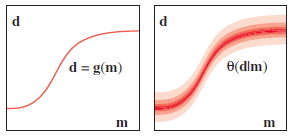
\includegraphics[width=.3\textwidth]{forwardmodel.png}
\end{figure}
The joint pdf (conditional times the marginal) gives the correlations of the physical theory together with its uncertainty. The marginal distribution is the homogenous pdf which characterise...
$$\Theta(\mathbf{d},\mathbf{m})=\theta(\mathbf{d \mid m}) \mu(\mathbf{m})$$


	\subsection{A priori information}
\begin{itemize}
	\item Prior measurement pdf: $\rho_D(\mathbf{d})$.
	\item Prior parameter pdf: $\rho_M(\mathbf{m})$.
\end{itemize}
The joint prior information is form by the two independent prior information 
$$\rho(\mathbf{d,m})=\rho_D(\mathbf{d}) \rho_M(\mathbf{m})$$


	\subsection{Inverse Problem}
The posteriori states of information is given by the conjuction of the theorical pdf $\Theta$ and prior pdf $\rho$. This can be consider as a very general eqution of inversion problem which simplify in most common form.
$$\sigma(\mathbf{d},\mathbf{m})=k\frac{\rho(\mathbf{d},\mathbf{m}) \Theta(\mathbf{d},\mathbf{m})}{\mu(\mathbf{d},\mathbf{m})}$$
k represent a normalization constant. 
\begin{figure}[H]
	\centering
	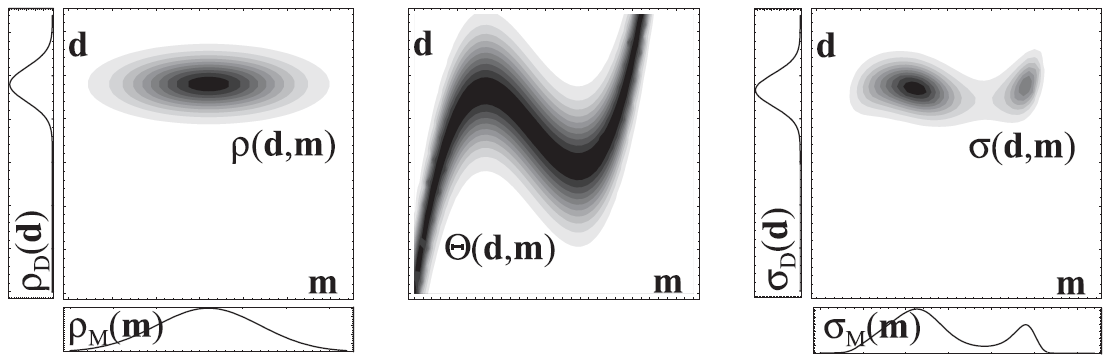
\includegraphics[width=.49\textwidth]{solution.png}
\end{figure}
The model parameter are updated with:
$$\boxed{\sigma_M(\mathbf{m})=\int_D\sigma(\mathbf{d},\mathbf{m})=k\rho_M(\mathbf{m})\int_D \frac{\rho_D(\mathbf{d})\theta(\mathbf{d \mid m}) }{\mu_D(\mathbf{d})}}$$
 

 
 



\newpage
\section{Least-Square Problem}
The least squares method approximate an overdetermined systems by minimizing the sum of the squares of the errors (L-2 norm, distance...etc).
Two following simplification are made (i) the data space is linear and therefore the homogeneous pdf $\mu_D(\mathbf{d})$ is constant and (ii) modelization uncertainty $\mathbf{C_T}$ are neglectable compare to observation uncertainty $C_D$. This second assumption imply that forward relation pdf is 0 every except in $\mathbf{d} = G(\mathbf{m})$ (the relation has no error):
$$\theta(\mathbf{d \mid m}) = \delta(\mathbf{d} - G(\mathbf{m}))$$

The model paramter pdf can be simplify:
$$\sigma_M(\mathbf{m}) \propto \rho_M(\mathbf{m})\int_D \rho_D(\mathbf{d}) \delta(\mathbf{d} - G(\mathbf{m}))\propto \rho_M(\mathbf{m}) \cdot \rho_D(G(\mathbf{m}))  $$

Least-square assume a Gaussian distribution for the priori unknown model parameter $\mathbf{m}$ and the observed measurement $\mathbf{d}$
$$\rho_M (\mathbf{m}) \sim \mathcal{N} (\mathbf{m^{prior}},\mathbf{C_M}) $$
$$\rho_D (\mathbf{d})=\rho_D (G(\mathbf{m})) \sim \mathcal{N} (\mathbf{d^{obs}},\mathbf{C_D})$$

The posteriori model parameters pdf become:
\begin{multline*}
\sigma_M(\mathbf{m})
	\propto \exp\Biggl\{  -\frac{1}{2} \biggl( (G(\mathbf{m})-\mathbf{d^{obs}})^\mathrm{T} \mathbf{C_D}^{-1} (G(\mathbf{m})-\mathbf{d^{obs}})\\
	+ (\mathbf{m}-\mathbf{m^{prior}})^\mathrm{T} \mathbf{C_M}^{-1} (\mathbf{m}-\mathbf{m^{prior}} )\biggr) \Biggr\}
\end{multline*}

The misfit function is defined
$$\boxed{2S(\mathbf{m})=\|G(\mathbf{m})-\mathbf{d^{obs}}\|_D^2 + \|\mathbf{m}-\mathbf{m^{prior}}\|_M^2}$$
``Least square'' comes from this this sum of square of the misfit function. Solving least square method will involved minimizing this function. This become an optimization problem
$$\operatorname*{arg\,min}_\mathbf{m}  S(\mathbf{m}) := \{\mathbf{m}^* \mid \forall \mathbf{m} : f(\mathbf{m}^*) \le f(\mathbf{m})\}.$$


This is equivalent to maximized the posteriori model parameter pdf (see maximum posteriori likelihood \ref{})

	\subsection{Linear least squares}
For linear problem $\mathbf{d=Gm}$, the misfit became quadratic (polynomial of degree 2). 
$$2S(\mathbf{m})=\|\mathbf{Gm}-\mathbf{d^{obs}}\|_D^2 + \|\mathbf{m}-\mathbf{m^{prior}}\|_M^2$$
It can be show (see \ref{•}) that this equation is equivalent to:
$$S(\mathbf{m})= (\mathbf{m-\tilde{m}})^\mathrm{T}  \mathbf{\tilde{C}_{M}^{-1}}  (\mathbf{m-\tilde{m}})$$
with:
$$\mathbf{\tilde{m}=(G^\mathrm{T}C_D^{-1}G+C_M^{-1})^{-1} (G^\mathrm{T}C_D^{-1}d^{obs}+C_M^{-1}m^{prior})}$$
$$\mathbf{\tilde{C}_M=(G^\mathrm{T}C_D^{-1}G+C_M^{-1})^{-1}}$$
And the misfit function is minimized for $\mathbf{m=\tilde{m}}$.


	\subsection{Ordinary least squares}
OLS assume zero or negligible errors in the independent variable $\mathbf{m=m^{prior}}$ and the misfit equation simplify to 
$$S(\mathbf{m})=\|\mathbf{Gm}-\mathbf{d^{obs}}\|_D^2$$

The most common approach is by setting the derivative of the misfit function to zero 
$$\frac{\partial S(\mathbf{m})}{\partial\mathbf{m}}=0$$
\begin{align*}
\nabla_\mathbf{m}(S) &=2\mathbf{ \nabla_\mathbf{m}(d^{obs}-Gm^{est})^\mathrm{T} C_D(d^{obs}-Gm^{est})} \\
					0&= 2\mathbf{G^\mathrm{T}C_D (d^{obs}-Gm^{est})}\\
					 \mathbf{G^\mathrm{T}C_Dd^{obs}}&=\mathbf{G^\mathrm{T}C_DGm^{est}}
\end{align*}



The predicted value will be:
$$  \mathbf{m^{est}=(G^\mathrm{T}C_DG)^{-1}G^\mathrm{T} C_D d^{obs} }$$
$$ \mathbf{d^{pred}=Gm^{est}=G(G^\mathrm{T}G)^{-1}G^\mathrm{T} d }$$
This can be view as a projection where $\mathbf{G(G^\mathrm{T}G)^{-1}G^\mathrm{T}}$ is the projection matrix and $\mathbf{G}$ is a matrix whose column vector  are a (not necessarily orthonormal) basis.

	\subsection{Constrainted Least-square}
The KKT (Kharush-Kuhn and Tucker) equations is used.The objective function is $f(\mathbf{x})=\|\mathbf{Ax-b}\|^2$, and the constraint function $\mathbf{Cx=D}$:
$$\Lambda(\mathbf{x},\lambda)=\|\mathbf{Ax-b}\|^2 + \sum \lambda_i( \mathbf{c}_i^T\mathbf{x}-d_i)$$

By searching the stationary point of the Lagrangian function $\frac{\partial \Lambda}{\partial x_i}=\frac{\partial \Lambda}{\partial \lambda_i}=0$ we find the following equations:
$$ 2\mathbf{A}^T(\mathbf{A\hat{x}-b})+\mathbf{C}^T\lambda =0 \qquad \mathbf{C\hat{x}+d}=0 $$
which can be re-written:
$$ \begin{bmatrix}
       2\mathbf{A}^T\mathbf{A} 	& \mathbf{C}^T \\
       \mathbf{C} 				& 0            \\
    \end{bmatrix} 
    \begin{bmatrix}
       \hat{\mathbf{x}}\\
       \mathbf{\lambda} 	\\
    \end{bmatrix}
    =
    \begin{bmatrix}
       2\mathbf{A}^T\mathbf{b}\\
       \mathbf{d} 	\\
    \end{bmatrix}
$$

	\subsection{Non-linear least square}
Two linearisation of $\mathbf{g(m)}$ are possible
\begin{enumerate}
	\item The weakest case is when it can be linearised around $m^{prior}$
	$$\mathbf{g(m)\approx g(m^{prior}) + G(m-m^{prior})}$$
	\item The second one is using maximum likelihood with an iterative method (eg. quasi-newton)
\end{enumerate}
\newpage



















\newpage
\section{Maximum Likelihood}
The likelihood of a set of parameter values, θ, given outcomes x, is equal to the probability of those observed outcomes given those parameter values, that is
$$\mathcal{L}(\mathbf{m} |\mathbf{d}) = P(\mathbf{d} | \mathbf{m}).$$


We will show that with a Gaussian prior and a linear forward model, the posteriori pdf is also Gaussian. Using \footnote{$\mathbf{x \sim \mathcal{N} (a,A)  \Rightarrow Ga \sim \mathcal{N} (Ga,G^\mathrm{T}AG)}$} and \footnote{$\mathbf{\mathcal{N} (a,A) \cdot \mathcal{N} (b,B)  \sim \mathcal{N} (c,C)}$ with $\mathbf{C=(A^{-1}+B^{-1})^{-1}}$ and $\mathbf{c=C(A^{-1}a + B^{-1}b)}$}
\begin{align*}
\sigma_M(\mathbf{m})& \propto  \rho_M(\mathbf{m}) \cdot \rho_D(\mathbf{Gm})\\
					& \propto  \mathbf{\mathcal{N}(m^{prior},C_M)  \cdot \mathcal{N} (G^{-1}d^{obs},(G^{-1})^\mathrm{T}C_DG^{-1})} \\
					& \sim  \mathcal{N} \mathbf{  (\tilde{m},\tilde{C}_M) }
\end{align*}

with 
$$\mathbf{\tilde{m}=(G^\mathrm{T}C_D^{-1}G+C_M^{-1})^{-1} (G^\mathrm{T}C_D^{-1}d^{obs}+C_M^{-1}m^{prior})}$$
$$\mathbf{\tilde{C}_M=(G^\mathrm{T}C_D^{-1}G+C_M^{-1})^{-1}}$$

	\subsection{Maximum Likelihood Estimate (MLE)}
The Maximum Likelihood Estimate (MLE) selects the parameters which maximized (the mode) the likelihood function a given statistical model.
\begin{align*}
\mathbf{\hat{m}_{MLE}}
&=\operatorname*{arg\,max}_\mathbf{m} p(\mathbf{d}\mid \mathbf{m})\\
&=\operatorname*{arg\,min}_\mathbf{m}  (\mathbf{d^{obs}}-G(\mathbf{m}))^\mathrm{T} \mathbf{C_D}^{-1} (\mathbf{d^{obs}}-G(\mathbf{m}))\\
\end{align*}
This is nothing more than the weighted least-squared method with the covariance matrix corresponding to the weighted matrix.

	\subsection{Maximum A Posteriori estimation (MAP)}
MAP assume that the parameter are drown from a random process (prior) and therefore it can be seen as a regularization (addition information) of MLE. This avoid over fitting of the data as the assumed (or known) prior knowledge bring back the estimate to its value.

$$\mathbf{\hat{m}_{MAP}}=\operatorname*{arg\,max}_\mathbf{m} p(\mathbf{m}\mid \mathbf{d})=  p(\mathbf{d}\mid \mathbf{m})  p(\mathbf{d})$$



\newpage
\section{More simplier way} 
 	\subsection{Probabilistic framework}
We can rephrase the problem in a simpler probabilistic manner: We observed some data which can be explain by the model and some white error $\boldsymbol \epsilon \sim \mathcal{N} (0,\mathbf{C_D})$
$$ \mathbf{d^{obs}} = G(\mathbf{m^{real}}) +\boldsymbol \epsilon$$
And therefore,
\begin{align*}
p(\mathbf{d^{obs}} \mid \mathbf{m} )
&\sim \mathcal{N} (G(\mathbf{m}),\mathbf{C_D})\\ 
&\propto \exp \left( -\frac{1}{2} (\mathbf{d^{obs}}-G(\mathbf{m}))^\mathrm{T} \mathbf{C_D}^{-1} (\mathbf{d^{obs}}-G(\mathbf{m})) \right)
\end{align*}

Using Bayes probability, the probability density of the parameter are updated with the observations data.
$$ p( \mathbf{m}\mid \mathbf{d^{obs}}) \propto p(\mathbf{d^{obs}} \mid \mathbf{m}) p(\mathbf{m})$$




	\subsection{Optimization}
We can modify further the problem to transform it into a optimization question. The objective function measure the mismatch between observed and simulated value and is minimized by optimization algorithm 
 $$\operatorname*{arg\,min}_\mathbf{m} OF( \mathbf{d^{obs}} - G(\mathbf{m}) )$$
 
 
 
 
	\subsection{Regularization}
Regularization introduces additional information in order to solve an ill-posed problem or to prevent overfitting. It is similar to adding a prior information in Bayesian point of view. 
 $$\operatorname*{arg\,min}_\mathbf{m} OF( \mathbf{d^{obs}} - G(\mathbf{m}) +R)$$

One common assumptions used as regulariation include:
\begin{itemize}
	\item Minimizing euclidean length of the solution $R=\mathbf{m}^\mathrm{T}\mathbf{m}$.
	\item Minimizing distance to a known value (eg. mean): $R=(\mathbf{m}-\mean{\mathbf{m}})^\mathrm{T}(\mathbf{m}-\mean{\mathbf{m}})$.
	\item Minimizing a linear function of the value (such as a flatness measure): $R=(D\mathbf{m})^\mathrm{T}(D\mathbf{m})=\mathbf{m}^\mathrm{T}D^\mathrm{T}D\mathbf{m}$. Where $D^\mathrm{T}D$ might be interpreted as a weighted factor. It could also be the difference matrix (measuring $\mathbf{x_i-x_{i-1}}$), in which case, we smooth the solution.
	\item Combining to last approach: $R=(\mathbf{m}-\mean{\mathbf{m}})^\mathrm{T}D^\mathrm{T}D(\mathbf{m}-\mean{\mathbf{m}})$
	\item 
\end{itemize}

For under-determined problem, regularisation methods are employed and the problem is solved with Lagrange where the regularisation is viewed as a constraint on the solution.


	\subsection{Resolution Matrix}
		\subsubsection{Data Resolution Matrix}
The Data Resolution Matrix $\mathbf{R_d}$ describe how well the the observed data describe the predicted data. 
$$\mathbf{d^{pred}=Gm^{est}=GG^{-1}d^{obs}=R_d d^{obs}}$$
If $\mathbf{R_d=I}$, the prediction error are zero. The ith row of the matrix describes how each observed data influence the ith predicted data (as a weighted sum). 

		\subsubsection{Model Resolution Matrix}
While the data resolution matrix characterizes whether the data can be independently predicted, the Model Resolution Matrix $\mathbf{R_m}$ related the true model parameter to the estimated one. If  $\mathbf{R_m=I}$, the model parameter is uniquely determined. The row of the matrix describe how well neighbouring data can be independently resolved.

$$\mathbf{m^{est}=G^{-1}d=G^{-1}Gm^{true}=R_m m^{true}}$$



		\subsubsection{Covariance Resolution Matrix}
The model covariance matrix is define as:
$$\mathbf{\text{Cov}(m^{est}) = G^{-1}\text{Cov}(d) G^{-1T}}$$


\newpage
\section{Solution}




	\subsection{Linear Problem: Invertible}
In case of an linear problem with an invertible matrix ($\exists \mathbf{A^{-1}} \mid  \mathbf{A^{-1}A=I}$), the problem become a matrix inversion problem ($\mathbf{m=G^{-1}d}$) which has a unique solution.


		\subsubsection{Back (Forward) substitution}
For upper (lower) triangular matrice, each coefficient can be computed from previous coefficient up to the last row ($U_{n,n}x_{n}=b_n$)
	$$x_i=\frac{b_n -\sum_{j=1}^{n-1} U_{i,j}x_j}{U_{i,i}}$$
For none-triangular matrix, the QR factorisation can be employ :

		\subsubsection{Factor and Solve methods}
This set of method refere to those which use first a decomposition in easily invertible matrix and then a solve the inverted matrix. The factor step is usually more computer expensive
	\begin{itemize}
		\item LU decomposition\hfill $\mathbf{A=LU}$ \\
		(1) forward substitution\hfill $\mathbf{Ly=b}$, with $\mathbf{y=Ux}$\\
		(2) a backward substitution \hfill$\mathbf{Ux=y}$.
		\item QR decomposition\hfill $\mathbf{A=QR \Rightarrow Rx=Q^\mathrm{T}b}$\\ 
		(1) compute y\hfill $\mathbf{y=Q^\mathrm{T}b}$\\
		(2) backward substitution \hfill$\mathbf{Rx=y}$
		\item Cholesky decomposition\hfill $\mathbf{A = LL^*}$,\\
		(1) Forward substitution\hfill $\mathbf{Ly = b}$ with $\mathbf{y=L^*x}$\\
		(2) Back substitution \hfill$\mathbf{L^*x = y}$
	\end{itemize}
	
		\subsubsection{Gauss elimination}
		\subsubsection{Cramer's rule}
For a nonzero determinant matrice $A$, the theorem state that the unique solution is
	$$ x_i = \frac{\det(A_i)}{\det(A)} \qquad i = 1, \ldots, n$$
where  $A_i$  is the matrix formed by replacing the i-th column of $A$ by the column vector $b$.


	\subsection{Linear Problem : not Invertible}
This become a linear regression which can be view as an optimization problem.

		\subsubsection{Pseudo-Inverse}
The pseudo-inverse (or Moore-Penrose Inverse) provides a least squares solution to a system of linear equations.
For full column rank (left invertible $ A^+A=I$), pseudo-inverse is computed by: $ A^+ = (A^* A)^{-1} A^*$ while for full row rank (right inverse): $ A^+ = A^* (A A^*)^{-1} $
		
		\subsubsection{Newton's method}
The model fonction $G(\mathbf{m})$ need to be 2 order differentiable ($\nabla_G$ and $\mathbf{H}_G$)





	\subsection{Non-linear Problem}
\subsubsection{Non-linear least square - Newton's Method}
The minimization of the general least-square problem with Newton's Method involved computing the Jacobien and Hessian of $S(\mathbf{m})$
Recall:
$$2S(\mathbf{m})=\|G(\mathbf{m})-\mathbf{d^{obs}}\|_D^2 + \|\mathbf{m}-\mathbf{m^{prior}}\|_M^2$$
$$\mathbf{J}_S(\mathbf{m})=\mathbf{J}_G\mathbf{C}_D^{-1}(G(\mathbf{m})-\mathbf{d^{obs}}) + \mathbf{C}_M^{-1} (\mathbf{m}-\mathbf{m^{prior}})$$
$$\mathbf{H}_S(\mathbf{m})=\mathbf{J}_G^\mathrm{T}\mathbf{C}_D^{-1}\mathbf{J}_G  + \mathbf{H}_G \mathbf{C}_D^{-1} (G(\mathbf{m})-\mathbf{d^{obs}}) + \mathbf{C}_M^{-1} $$

where $\mathbf{J}_G(\mathbf{m})=\mathbf{J}_{i,j}=\frac{\partial G(\mathbf{m})_i}{\partial m_j}$ and $\mathbf{H}_G(\mathbf{m})=\mathbf{H}_{i,j}=\frac{\partial G(\mathbf{m})}{\partial m_i \partial m_j}$ (?)

In the Gaussian-Newton Method, the second term of the Hessian (involving the Hessian of G) can be neglected.

The interative process become:
$$\mathbf{m}_{n+1} = \mathbf{m}_{n} - \frac{\mathbf{J}_S}{\mathbf{H}_S}$$

\bibliographystyle{apalike}
\bibliography{citations}	
	

\end{document}
